\chapter{向前走} \label{chap:chap12}


我们必须有意识地走完通往目标的路程的一部分,然后在黑暗中迈向成功。
\begin{flushright}
	——亨利$\cdot$戴维$\cdot$梭罗
\end{flushright}


\begin{figure}[!htb]
	\centering
	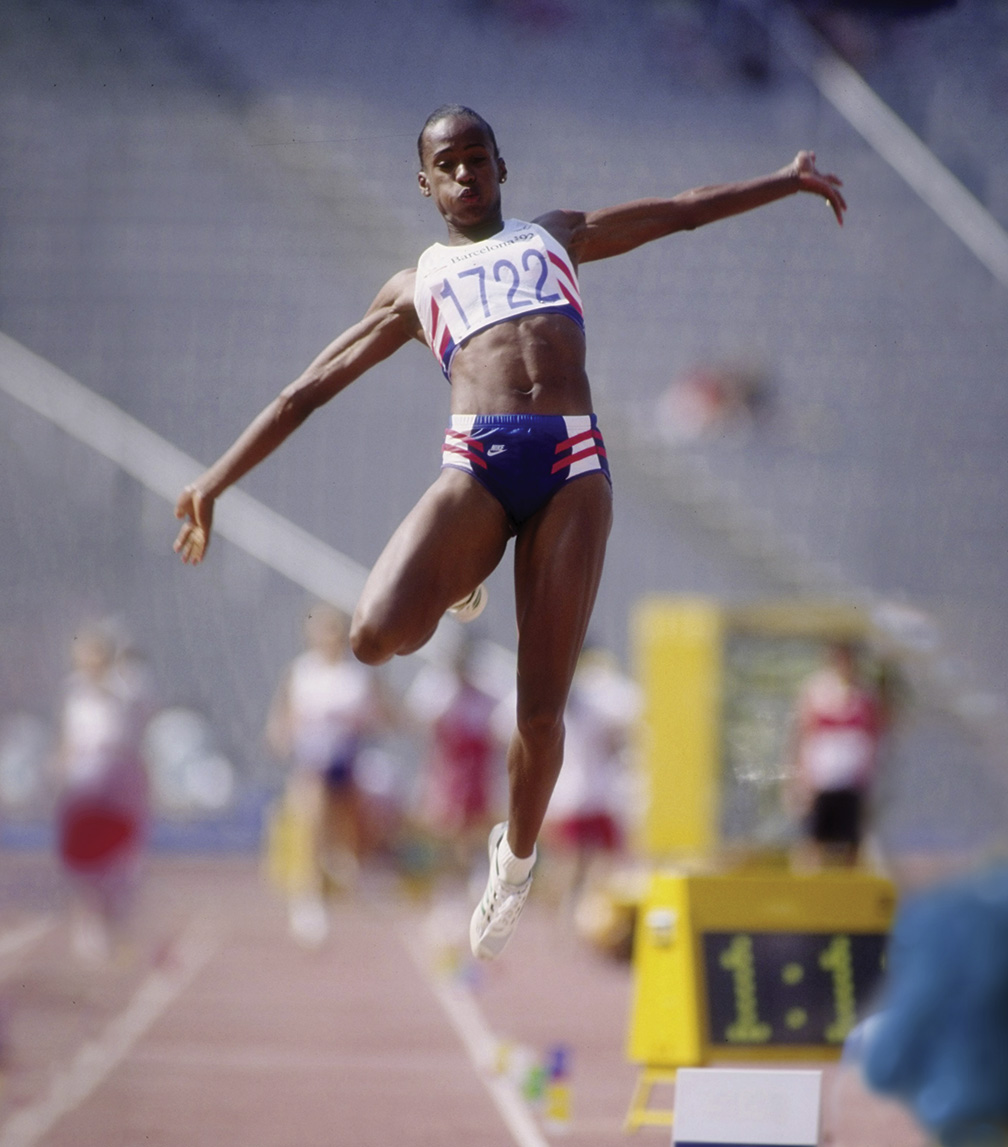
\includegraphics[width=1.0\linewidth]{chap13/13_0}
	% 加星号(*)表示不加编号
	\caption*{ \label{fig:13_0}}
\end{figure}

运动生物力学领域取得了长足的进步,但仍有更多领域有待探索。
本书介绍了测量、模型和计算工具如何帮助我们理解人类运动。
我们还展示了生物力学模型如何应用于机器人、跑道和外骨骼的设计。
生物力学使我们能够设计保护工人免受伤害的工厂,并制造出关节置换装置,使患有关节疾病的患者能够无痛行走。


这些成就改善了数百万人的生活,但我们也必须意识到现有知识和技术的局限性。
科技的新发展将使我们能够对人们的生活产生进一步的积极影响;
假肢功能的日益增强就是一个很好的例子。
知识的局限性更难克服。
克服这些局限性最重要的是,我们需要创造力,以及正如梭罗所说,勇于探索的勇气。


我想以我的一位合作者取得巨大成功的一次创造性飞跃作为本章的开篇。
接下来,我将描绘一幅我对生物力学领域的未来愿景——这幅愿景当然并不完整。
你的远见卓识将为这幅充满可能性的画布增添色彩和质感,在那里,你将拥有无限的空间去创造你的杰作。


\section{可穿戴技术}

凯特$\cdot$罗森布鲁斯在我的实验室工作时,在斯坦福医院遇到了一位男士,他因为一种叫做特发性震颤的疾病而无法给妻子写便条,也无法和朋友喝咖啡。
这是一种极其令人沮丧的疾病,但却非常常见。
五六十岁患上特发性震颤的人会因为手抖而无法进行日常生活活动。


这位患有特发性震颤的男子告诉凯特,他尝试过的药物并没有减轻他的手部震颤,而且副作用很大。
他唯一的选择就是手术,在脑部植入刺激电极。
这种疗法被称为深部脑刺激,已被证明对减轻震颤非常有效,但需要进行脑部手术。
脑部手术有严重并发症的风险。
这不是一个可以轻易做出的决定。


凯特知道,他的手颤抖很可能是由大脑特定区域的震荡神经活动引起的,其中包括丘脑腹侧中间核。
凯特找到一些文章,表明电刺激腕部正中神经会引发腹侧中间核内的神经活动。
她推断,刺激腕部的感觉神经或许能激发该脑区活动,从而无需手术即可减轻手部震颤。
作为一项实验,她决定尝试刺激几位自愿接受治疗的特发性震颤患者的正中神经。


这简直是​​一次盲目的尝试。
我们尚不清楚大脑震荡神经活动的确切原因,也不知道腕部电刺激是否会影响它。
但令我们(以及我们的参与者)欣喜的是,刺激正中神经后,他们的手部震颤显著减少。
这些初步数据激励着我们继续前进。
我们继续实验并学习这项新技术。
例如,当以与震颤相同的频率刺激正中神经时,我们发现效果最佳。
凯特与塞雷娜$\cdot$黄(Serena Wong)等人合作,打造了一款可穿戴运动传感器和神经刺激器,其外形类似腕表,可以记录患者手部震颤的频率,并以震颤频率刺激腕部神经。
令人欣慰的是,许多使用该设备的人的手部震颤显著减少\cite{lin2018noninvasive}。
他们恢复了写便条、喝咖啡以及进行其他用握手无法进行的活动的能力(图~\ref{fig:13_1})。


\begin{figure}[!htb]
	\centering
	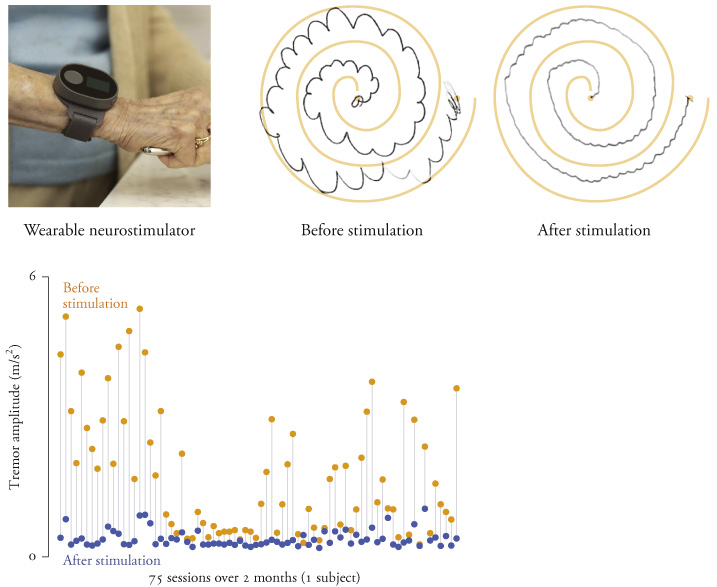
\includegraphics[width=1.0\linewidth]{chap13/13_1}
	\caption{可穿戴运动传感器和神经刺激器可减少手部震颤。
		Cala Health 的一款可穿戴刺激器(左上)显著减少了手部震颤(下图)。
		一位患者在接受 40 分钟神经刺激治疗后,螺旋画法显著改善(右上)。
		Cala Health, Inc. 是一家斯坦福大学衍生公司,由 Kate Rosenbluth、Serena Wong 和 Scott Delp 共同创立。 \label{fig:13_1}}
\end{figure}


这种新疗法无需药物和手术即可减轻手部震颤。
凯特的创造力和小型惯性测量单元使这项技术成为可能,这些单元可以记录患者的手部运动,使我们能够确定个性化的刺激模式。
神经刺激的效果,以及饮用咖啡或酒精(这些因素会影响手部震颤的程度)和其他因素的影响,可以在患者日常生活中持续数月进行监测。
未来,我们设想成千上万的患者佩戴神经刺激器,记录他们的手部运动并监测治疗效果,从而优化每位患者的功能。


小规模运动传感技术为推进治疗和研究提供了更多机遇。
目前,大多数生物力学实验都是在受控的实验室环境中使用本书所述的技术进行的。
但实验室测量存在严重的局限性。
例如,用于规划脑瘫儿童手术的步态分析通常依赖于在实验室这个陌生环境中仅测量几步的步数,这可能无法代表儿童在日常生活中的能力。
既然我们能够测量实验室外的运动,就可以开始使用在日常生活中几个月内测量的数千步步数来规划治疗方案。
我希望这能帮助我们做出更好的手术决策。


小型传感设备仍有很大改进空间。
目前可穿戴运动监测方法的精度不足以满足许多应用需求,尤其是在涉及运动模式受损人群的应用,准确区分功能性运动和症状性运动至关重要。
现实世界中,长时间佩戴传感器进行生物力学测量会产生大量噪声数据,我们需要新的方法来从这些海量数据集中获取洞见。
这为数据科学和生物力学领域的从业者提供了一个进行有意义互动的机会。


\section{随处可见的物理康复}

行走能力是独立生活的标志。
然而,中风、帕金森病和脑瘫等神经系统疾病和损伤严重限制了人们的活动能力。
骨关节炎等肌肉骨骼疾病会引发疼痛,并限制数百万人的行动能力。
总的来说,行动不便的后果广泛而严重。


康复对于改善行动障碍人士的生活至关重要。
多年来,我在康复诊所工作,深受人们渴望重拾能力的动力以及指导他们康复的治疗师的精湛技艺的鼓舞。
然而,目前的康复方法依赖于诊所内的评估和治疗。
物理治疗师和职业治疗师会评估患者并制定治疗方案,但他们缺乏衡量患者在诊所外活动能力的工具,也缺乏利用数百名类似患者数据来制定治疗方案的方法。
患者需要前往诊所就诊,加上高昂的治疗费用,限制了那些努力康复的患者能够获得的治疗数量。


我们必须开发工具,让患者无需前往诊所即可参与康复。
如果力量训练和活动训练可以在家进行,那么它们的开展频率就会更高。
移动传感器可以测量运动,但提供的信息并不完整。
我们还需要能够应用先进生物力学模型的软件,以精准量化行动障碍患者的运动。
通过优化这些工具,使其能够在智能手机上运行,​​并提供触觉、听觉和视觉反馈,我们可以将智能手机转变为运动测量系统和虚拟物理治疗师。
此外,机器学习方法可以从数千篇科学论文和描述数百万个体的数据(包括视频、临床记录和来自移动传感器的信号)中提取洞见,从而有可能以低成本提供有价值的指导。
对于我们这个领域来说,如何开发这些技术,使其能够为行动障碍患者带来切实的益处,而不是仅仅为了技术而开发技术,这将是一个挑战。


\subsection{大规模实验}

我做过的大多数研究都只有几十名参与者。
几年前,随着全球一些最大的公司开始对生物力学产生兴趣,数百万人开始携带配备运动传感器的智能手机,情况发生了改变。
我曾梦想能够进行大规模的实验。
随着全球大部分人口的手机都配备了加速度计,这个梦想或许可以成为现实。


我和我的合作伙伴与当地一家初创公司 Azumio Inc. 合作,收集并分析了来自 46 个国家/地区的 60 多万人的基于智能手机传感器的活动模式,这使得这次调查成为规模最大的体育活动调查,规模大约是前者的 1,000 倍。
我们发现,人群中活动最少和最活跃群体之间的不平等可以预测每个人群的肥胖患病率(图~\ref{fig:13_2})。
活动不平等用基尼系数计算,该公式也用于计算收入不平等。
基尼系数的范围从 0(每个人都获得平等的资源份额(完全平等))到 1(一个人获得所有资源)。
在活动不平等严重的国家,通常是因为大量女性相对不活跃;
在这些人群中,女性的预期寿命较低。
我们发现,在步行条件更好的城市,例如餐馆离住所和工作场所都在步行距离内的城市,活动不平等程度较低。
在这些适合步行的城市中,女性的体育活动增幅最大。
这些发现表明,城市规划和公共卫生政策应侧重于增加那些活动量最少的人群的活动量。
我建议生物力学家参与城市和社区规划,将体育锻炼融入日常生活。
这将对数百万人的健康产生巨大的积极影响。


\begin{figure}[!htb]
	\centering
	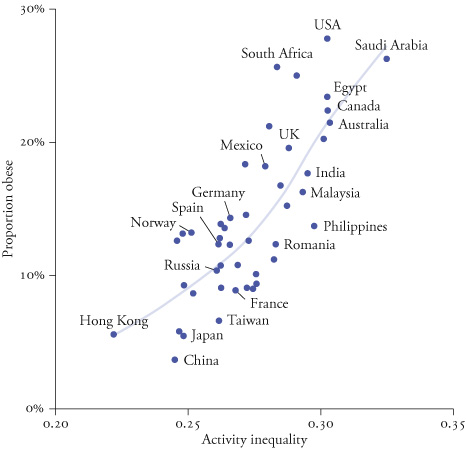
\includegraphics[width=0.75\linewidth]{chap13/13_2}
	\caption{活动不平等预测肥胖。
		活动不平等程度最高的五个国家/地区的个人肥胖可能性比活动不平等程度最低的五个国家/地区的个人高出196\% \cite{althoff2017large}。 \label{fig:13_2}}
\end{figure}








